% 例 3：平行四边形 ABCD 中心对称，对称中心 O = AC∩BD；P∈AB ↔ P'∈CD
\documentclass[tikz,border=4pt]{standalone}
\usepackage{ctex}
\usepackage{amsmath}
\usetikzlibrary{calc, decorations.markings}
\begin{document}
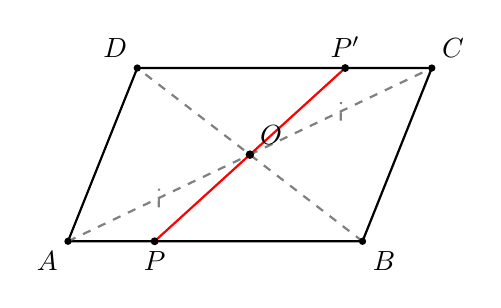
\begin{tikzpicture}[scale=1.1, thick,
  tickone/.style={postaction={decorate, decoration={markings,
    mark=at position 0.5 with {\draw (-1.5pt,-3pt) -- (1.5pt,3pt);}}}}]
  \coordinate (A) at (0,0);
  \coordinate (B) at (3.4,0);
  \coordinate (C) at (4.2,2);
  \coordinate (D) at (0.8,2);
  \coordinate (O) at (2.1,1);
  % P 在 AB 上：取 P=(1.0, 0)
  \coordinate (P) at (1.0, 0);
  % P' 是 P 关于 O 的对称点：P' = 2O - P = (3.2, 2) (在 CD 上)
  \coordinate (Pp) at (3.2, 2);

  \draw (A) -- (B) -- (C) -- (D) -- cycle;
  \draw[gray, dashed, tickone] (A) -- (O);
  \draw[gray, dashed, tickone] (O) -- (C);
  \draw[gray, dashed] (B) -- (D);
  \draw[red, thick] (P) -- (O) -- (Pp);

  \fill (A) circle (1.2pt); \fill (B) circle (1.2pt);
  \fill (C) circle (1.2pt); \fill (D) circle (1.2pt);
  \fill (O) circle (1.4pt);
  \fill (P) circle (1.3pt); \fill (Pp) circle (1.3pt);

  \node[below left] at (A) {$A$};
  \node[below right] at (B) {$B$};
  \node[above right] at (C) {$C$};
  \node[above left] at (D) {$D$};
  \node[above right] at (O) {$O$};
  \node[below] at (P) {$P$};
  \node[above] at (Pp) {$P'$};
\end{tikzpicture}
\end{document}
